\chapter{適用例}\label{cha:Indication}

本章では、本研究で試作した \tool が正しく動作することを、適用例を用いて確認する。
\tool{} は、\ref{sec:reqspec}節および\ref{sec:testcase}節で述べた、入力対象の要求仕様書とテストスイートに対して、
TCVダイアグラム(\ref{sec:testcase_visualization_diagram}節参照)を出力する。

\tool{}が出力するTCVダイアグラムによって、テストケースの可視化が正しく行えることを確認するために、
以下の2つの場合について確認する。

\begin{itemize}
    \item テストケースの抜けや不備または過剰箇所が存在する場合の確認
    \item テストケースの抜けや不備または過剰箇所が存在しない場合の確認
\end{itemize}

適用対象として、「閏年判定プログラム」を題材に、要求仕様書とテストスイートを作成した。
なお、テストスイートは、事前にテストケースの抜けや不備、過剰箇所を含めた状態で作成した。

作成した要求仕様書を図\ref{fig:reqspec}に、テストスイートを図\ref{fig:testsuite_1}、図\ref{fig:testsuite_2}に、それぞれ示す。

\begin{figure}[tp]                                                                            
    \begin{center}                                                                            
        \fbox{                                                                                
        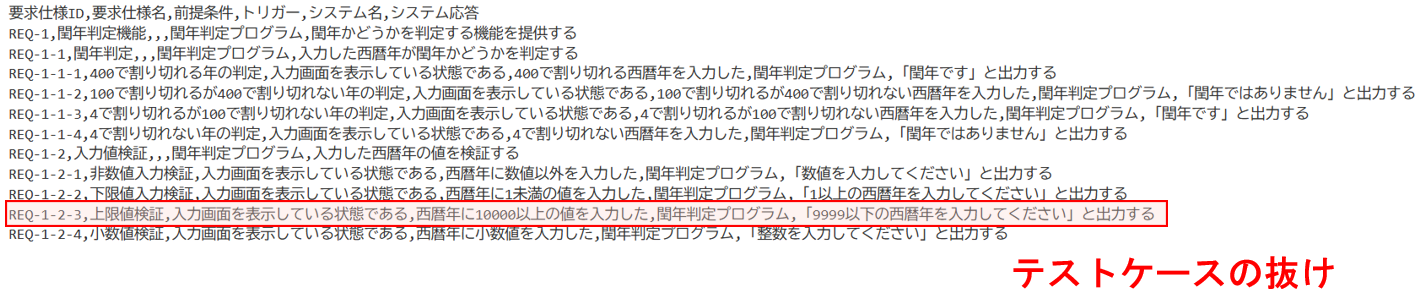
\includegraphics[width=0.96\textwidth]{images/05/reqspec.png}                 
        }                                                                                     
        \caption{作成した要求仕様書}                                              
        \label{fig:reqspec}                                                        
    \end{center}                                                                              
\end{figure}                                                                                  

\begin{figure}[tp]                                                                            
    \begin{center}                                                                            
        \fbox{                                                                                
        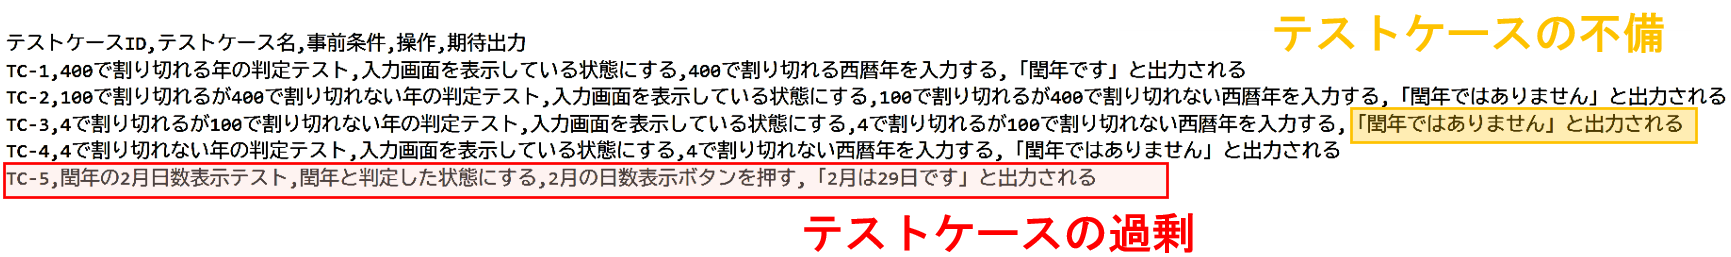
\includegraphics[width=0.96\textwidth]{images/05/testsuite_1.png}             
        }                                                                                     
        \caption{作成したテストスイート(入力形式検証テスト.csv)}                
        \label{fig:testsuite_1}                                                    
    \end{center}                                                                              
\end{figure}                                                                                  

\begin{figure}[tp]                                                                            
    \begin{center}                                                                            
        \fbox{                                                                                
        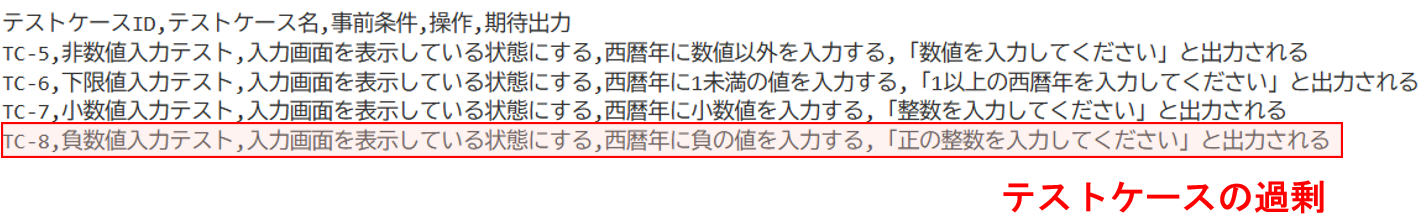
\includegraphics[width=0.96\textwidth]{images/05/testsuite_2.png}             
        }                                                                                     
        \caption{作成したテストスイート(閏年判定テスト.csv)}                      
        \label{fig:testsuite_2}                                                    
    \end{center}                                                                              
\end{figure}                                                                                  

\tool{} 実行時、初期設定(\ref{sec:config}節参照)で記述した設定ファイルvitt.yamlの処理設定(processing)に関する項目を、図\ref{fig:setting_sample1}に示す。

\begin{figure}[t]
    \setbox0\vbox{
        \vbox{processing:}
        \vbox{\ \ \ \ similarity\_threshold: 0.7}
        \vbox{\ \ \ \ weights:}
        \vbox{\ \ \ \ \ \ \ \ precondition: 0.2}
        \vbox{\ \ \ \ \ \ \ \ trigger\_operation: 0.4}
        \vbox{\ \ \ \ \ \ \ \ response\_output: 0.4}
	}
	\centerline{\fbox{\box0}}
    \caption{vitt.yaml}
    \label{fig:setting_sample1}
\end{figure}

% テストケースの抜けや不備または過剰箇所が存在する場合の確認
\section{テストケースの抜けや不備または過剰箇所が存在する場合の確認}\label{sec:indication_inconsistency}

本節では、テストケースの抜けや不備、過剰箇所が存在する場合の入力を\tool{} に適用し、出力するTCVダイアグラムを確認する。 

具体的には、TCVダイアグラムが以下の7点を満たすことを確認する。

\begin{itemize}                                                                             
    \item 要求仕様の矩形要素を、品質種別に対応する赤色(NONE)で表示し、テストケースの抜け箇所を強調していること。                       
    \item 要求仕様の矩形要素とテストケースの矩形要素の2つを、品質種別に対応する黄色(PARTIAL)で表示し、テストケースの不備箇所を強調していること。                  
    \item テストケースの矩形要素を、品質種別に対応する赤色(NONE)で表示し、テストケースの過剰箇所を強調していること。                                       
    \item 対応関係がある要求仕様の矩形要素とテストケースの矩形要素の2つを、品質種別に対応する緑色(FULL)で表示していること。
    \item 対応関係がある要求仕様の矩形要素とテストケースの矩形要素の2つを、点線で接続し、類似度の閾値以上の合計スコアをラベルとして付与していること。
    \item 対応付け可能ではない要求仕様の矩形要素を、品質種別に対応する白色(UNTRACEABLE)で表示していること。
    \item 子要求仕様の矩形要素から親要求仕様の矩形要素へ向かう矢印を描画していること。
\end{itemize}

図\ref{fig:testsuite_1}、図\ref{fig:testsuite_2}に示したテストスイートには、以下のテストケースの抜けや不備、過剰箇所が存在する。

\begin{itemize}                                                 
    \item テストケースの抜け \\
    要求仕様REQ-1-2-3と対応関係があるテストケースが存在しない。                                                                              
    \item テストケースの不備 \\
    テストケースTC-3の期待出力を表す文章『「閏年ではありません」と出力される』と、
    対応関係がある要求仕様REQ-1-1-3のシステム応答を表す文章『「閏年です」と出力する』とで出力内容が異なっており、
    テストケースの内容が不十分である。                  
    \item テストケースの過剰 \\
    テストケースTC-8と対応関係がある要求仕様が存在しない。                
\end{itemize}                                                                             

\tool{} が、図\ref{fig:reqspec}の要求仕様書と、図\ref{fig:testsuite_1}、図\ref{fig:testsuite_2}の
テストスイートを入力した際に出力するTCVダイアグラムを、図\ref{fig:tcv_inconsistency}に示す。   

\begin{figure}[tp]                                                                            
    \begin{center}                                                                            
        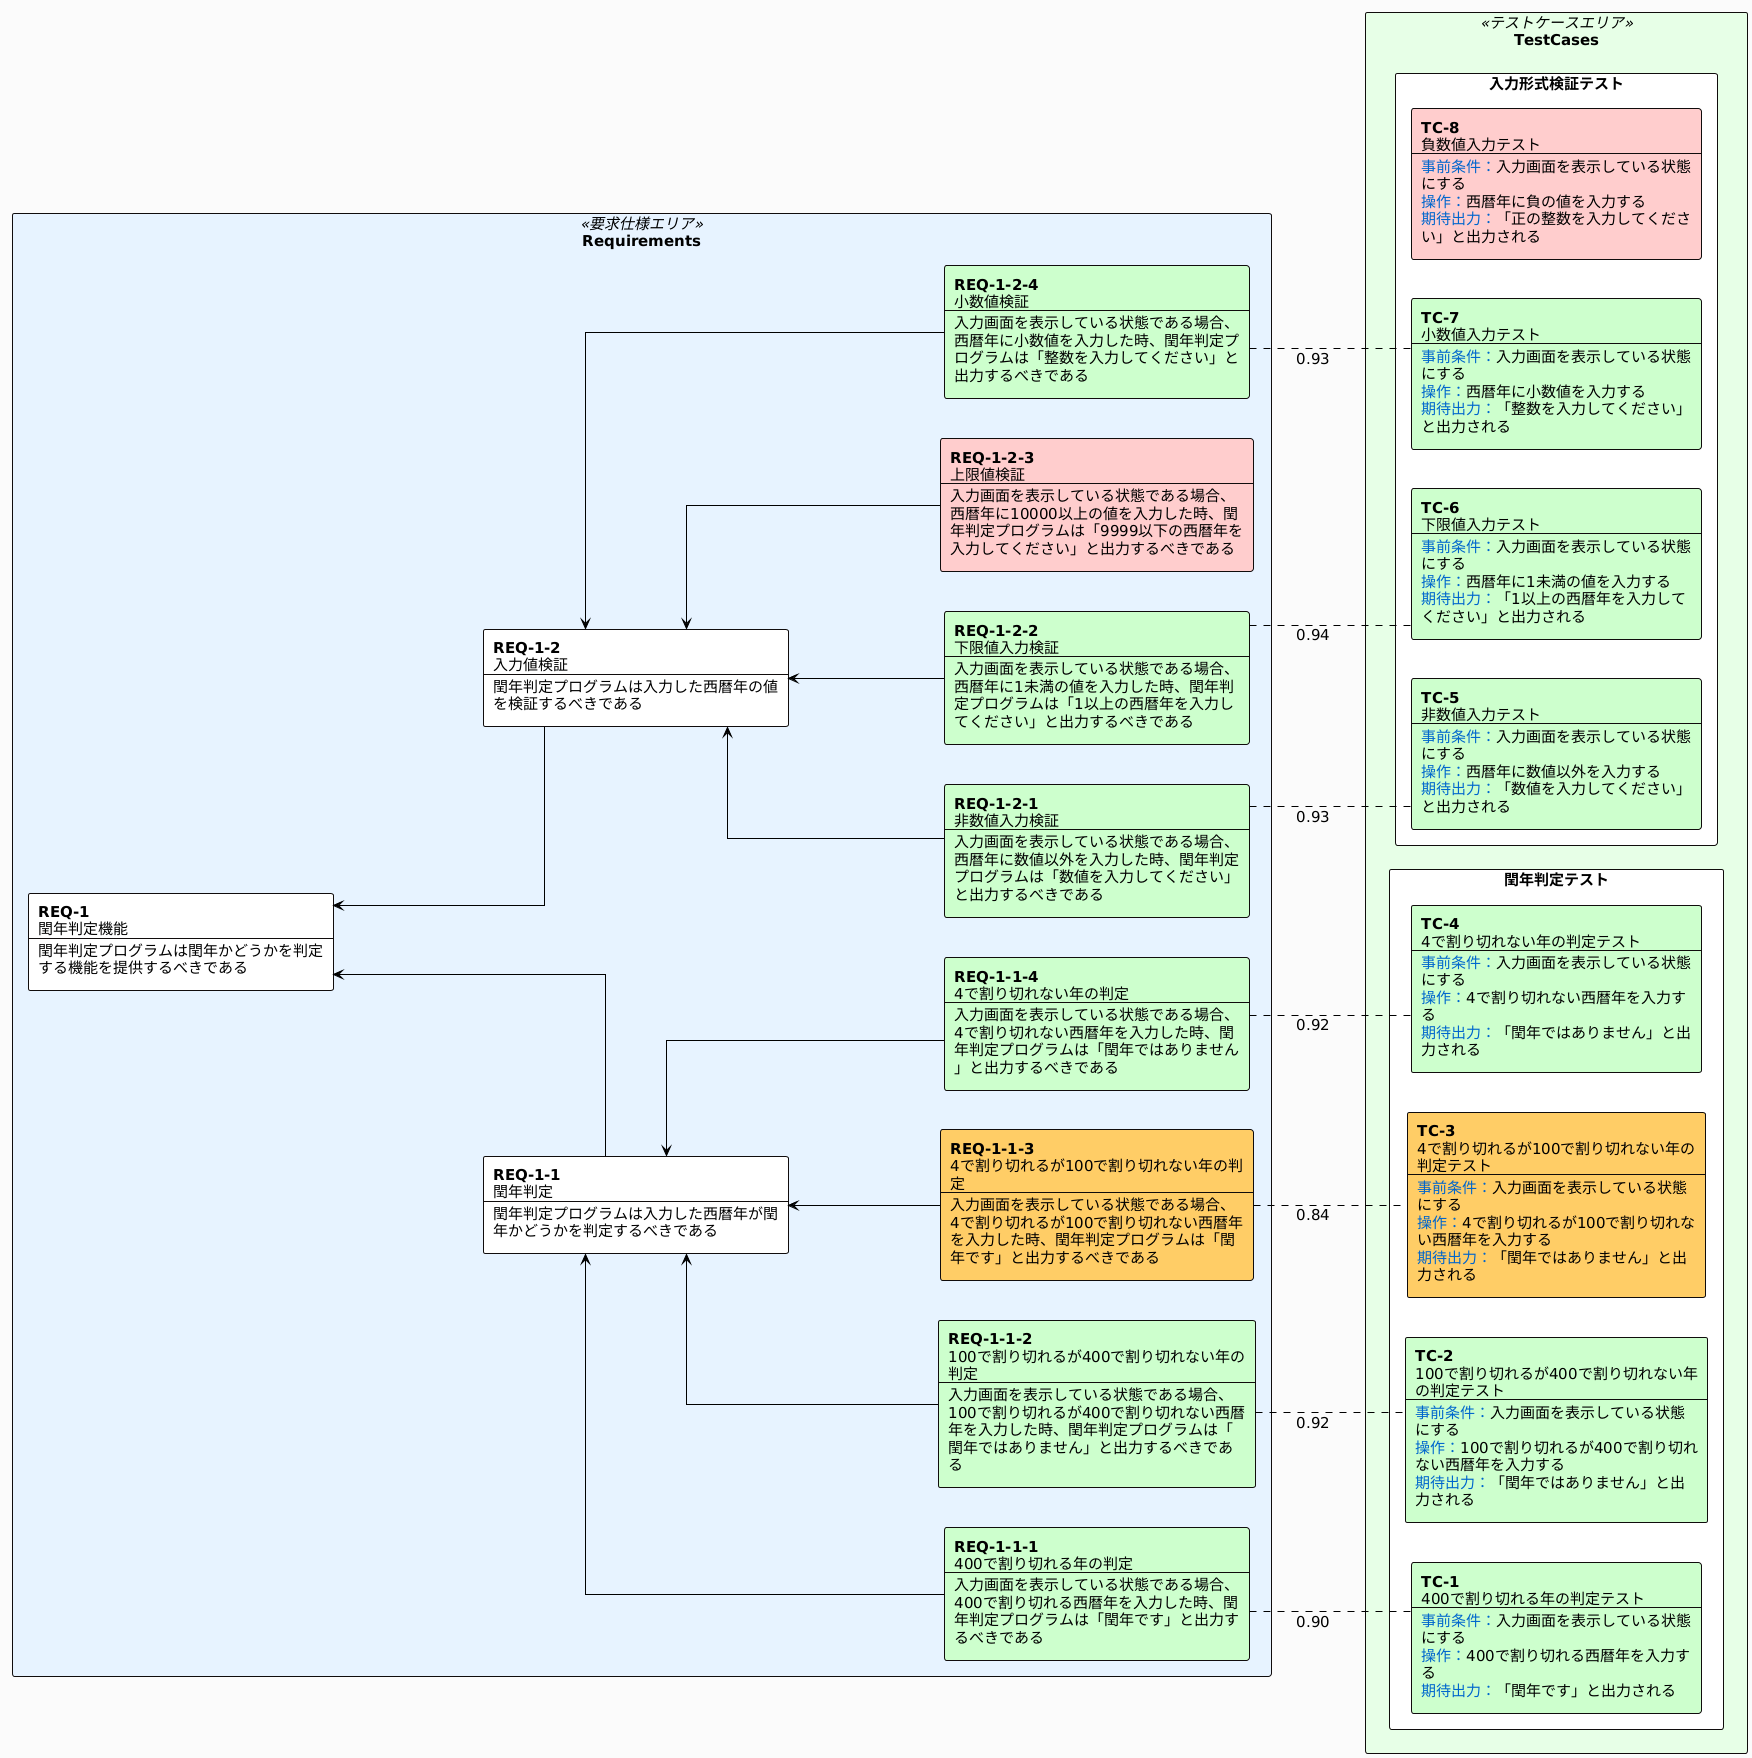
\includegraphics[width=17cm]{images/05/tcv_inconsistency.png}                 
        \caption{テストケースの抜けや不備または過剰箇所が存在する場合のTCVダイアグラム}       
        \label{fig:tcv_inconsistency}                                              
    \end{center}                                                                              
\end{figure}

図\ref{fig:tcv_inconsistency}より、出力したTCVダイアグラムが、以下の7点を満たすことを確認できた。

\begin{itemize}                                                                             
    \item 要求仕様REQ-1-2-3の矩形要素を、品質種別に対応する赤色(NONE)で表示し、テストケースの抜け箇所を強調していること。
    \item 要求仕様REQ-1-1-3の矩形要素とテストケースTC-3の矩形要素の2つを、品質種別に対応する黄色(PARTIAL)で表示し、テストケースの不備箇所を強調していること。
    \item テストケースTC-8の矩形要素を、品質種別に対応する赤色(NONE)で表示し、テストケースの過剰箇所を強調していること。
    \item 対応関係がある要求仕様の矩形要素とテストケースの矩形要素の2つを、品質種別に対応する緑色(FULL)で表示していること。
    \item 対応関係がある要求仕様の矩形要素とテストケースの矩形要素の2つを、点線で接続し、類似度の閾値0.7以上の合計スコアをラベルとして付与していること。
    \item 対応付け可能ではない要求仕様(REQ-1、REQ-1-1、REQ-1-2)の矩形要素を、品質種別に対応する白色(UNTRACEABLE)で表示していること。
    \item 子要求仕様の矩形要素から親要求仕様の矩形要素へ向かう矢印を描画していること。
\end{itemize}

% テストケースの抜けや不備または過剰箇所が存在しない場合の確認
\section{テストケースの抜けや不備または過剰箇所が存在しない場合の確認}\label{sec:indication_ground_truth}

本節では、テストケースの抜けや不備または過剰箇所が存在しない場合の入力を\tool{}に適用し、出力するTCVダイアグラムを確認する。

具体的には、TCVダイアグラムが以下の4点を満たすことを確認する。

\begin{itemize}                                                                             
    \item すべての対応付け可能な要求仕様の矩形要素とテストケースの矩形要素の2つを、品質種別に対応する緑色(FULL)で表示していること。
    \item 対応関係がある要求仕様の矩形要素とテストケースの矩形要素の2つを、点線で接続し、類似度の閾値以上の合計スコアをラベルとして付与していること。
    \item 対応付け可能ではない要求仕様の矩形要素を、品質種別に対応する白色(UNTRACEABLE)で表示していること。
    \item 子要求仕様の矩形要素から親要求仕様の矩形要素へ向かう矢印を描画していること。                                        
\end{itemize}

\ref{sec:indication_inconsistency}節で特定した、テストケースの抜けや不備、過剰箇所に対して、
修正した要求仕様書を図\ref{fig:reqspec_fixed}に、修正したテストスイートを図\ref{fig:testsuite_fixed_1}、図\ref{fig:testsuite_fixed_2}に、それぞれ示す。

\begin{figure}[tp]
    \begin{center}
        \fbox{
        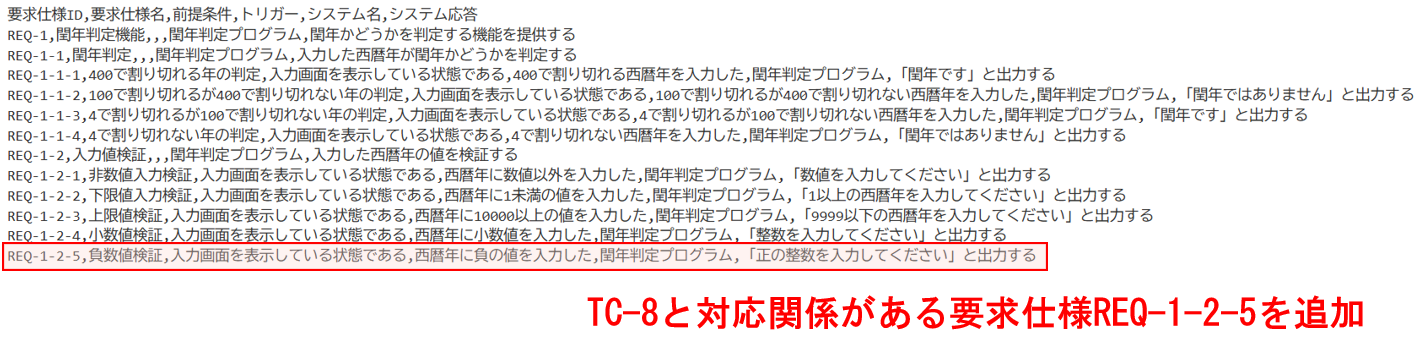
\includegraphics[width=0.96\textwidth]{images/05/reqspec_fixed.png}
        }
        \caption{修正した要求仕様書}
        \label{fig:reqspec_fixed}
    \end{center}
\end{figure}

\begin{figure}[tp]
    \begin{center}
        \fbox{
        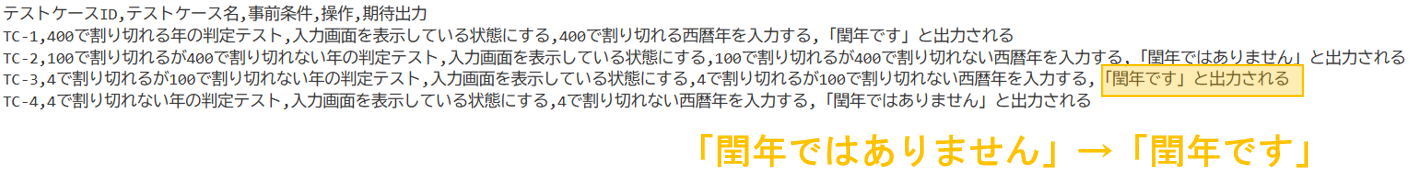
\includegraphics[width=0.96\textwidth]{images/05/testsuite_fixed_1.png}
        }
        \caption{修正したテストスイート(入力形式検証テスト.csv)}
        \label{fig:testsuite_fixed_1}
    \end{center}
\end{figure}

\begin{figure}[tp]
    \begin{center}
        \fbox{
        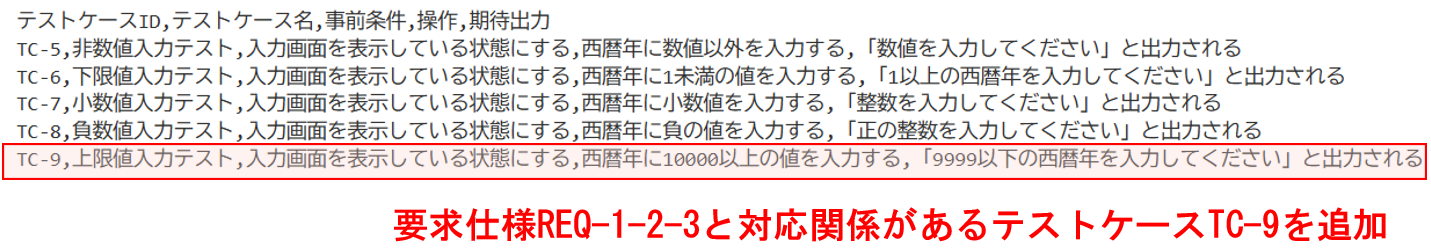
\includegraphics[width=0.96\textwidth]{images/05/testsuite_fixed_2.png}
        }
        \caption{修正したテストスイート(閏年判定テスト.csv)}
        \label{fig:testsuite_fixed_2}
    \end{center}
\end{figure}

具体的には、テストケースの抜けや不備、過剰箇所に対して、以下の修正を行った。

\begin{itemize}                                                 
    \item テストケースの抜け \\
    要求仕様REQ-1-2-3と対応関係があるテストケースが存在しなかったため、テストケースTC-9を追加した。                                                                              
    \item テストケースの不備 \\
    テストケースTC-3の期待出力が、対応関係がある要求仕様REQ-1-1-3のシステム応答と一致しなかったため、期待出力を『「閏年です」と出力される』に修正した。
    \item テストケースの過剰 \\
    テストケースTC-8と対応関係がある要求仕様が存在しなかったため、要求仕様REQ-1-2-5を追加した。
\end{itemize}

\tool{}が、図\ref{fig:reqspec_fixed}の要求仕様書と図\ref{fig:testsuite_fixed_1}、図\ref{fig:testsuite_fixed_2}のテストスイートを入力した際に出力するTCVダイアグラムを、図\ref{fig:tcv_ground_truth}に示す。

\begin{figure}[tp]
    \begin{center}
        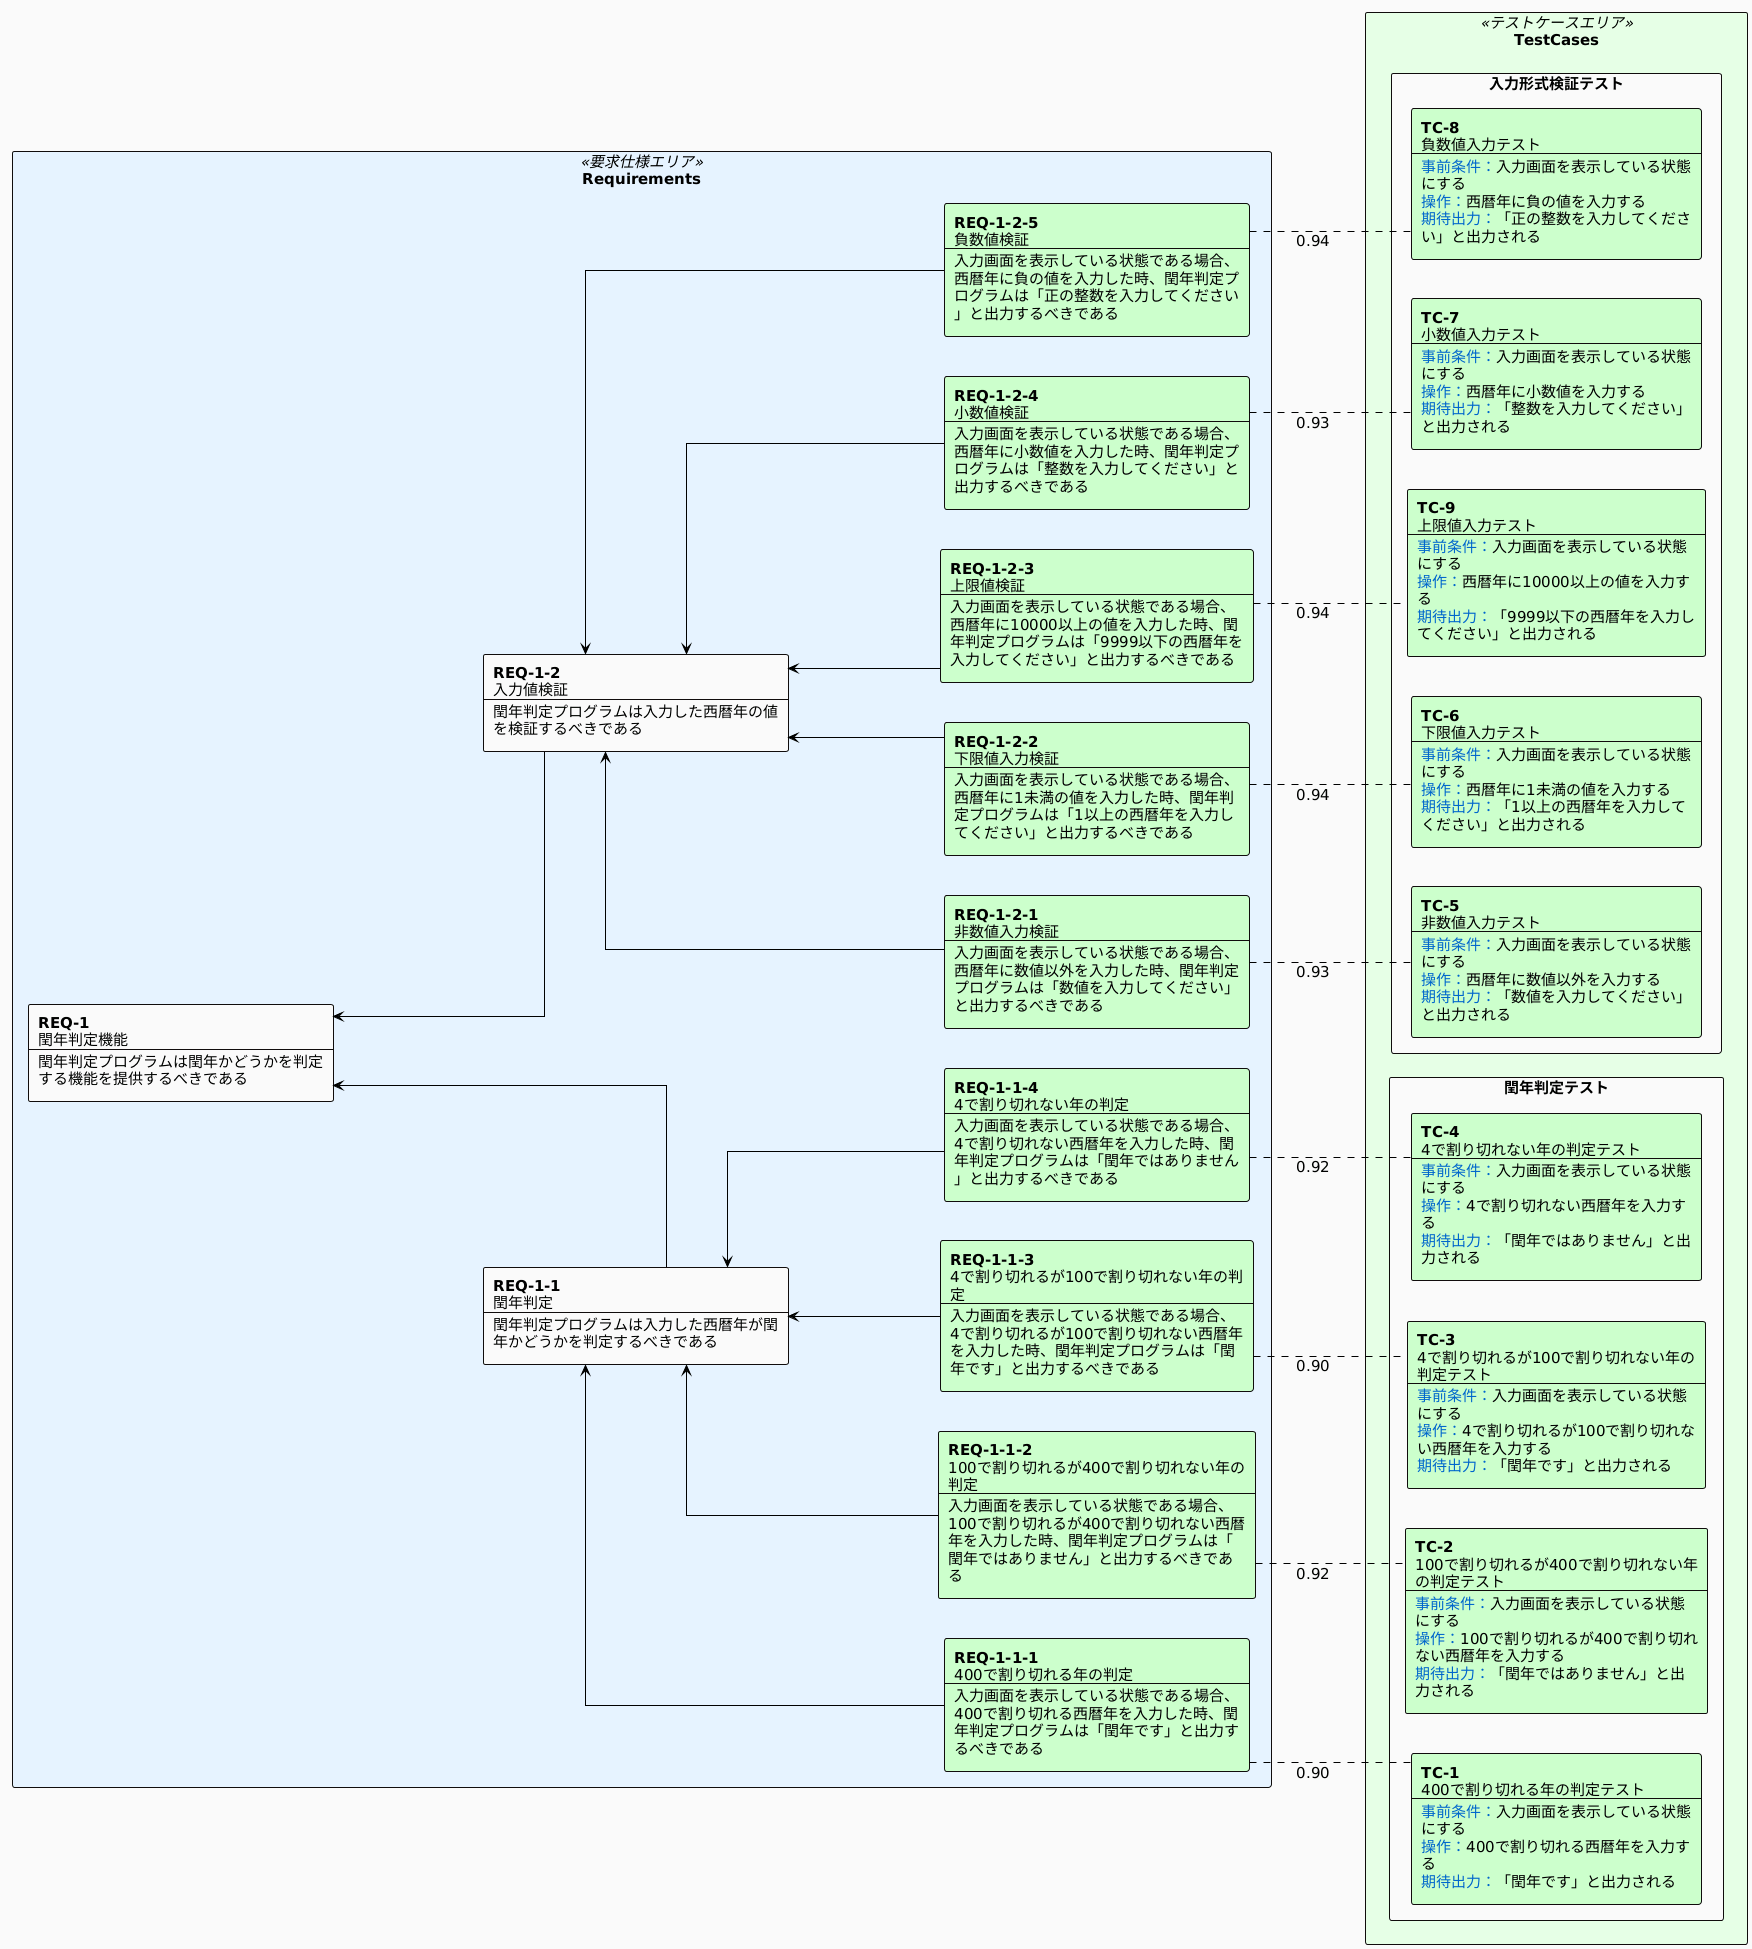
\includegraphics[width=17cm]{images/05/tcv_ground_truth.png}
        \caption{テストケースの抜けや不備または過剰箇所が存在しない場合のTCVダイアグラム}
        \label{fig:tcv_ground_truth}
    \end{center}
\end{figure}

図\ref{fig:tcv_ground_truth}より、出力したTCVダイアグラムが、以下の4点を満たすことを確認できた。

\begin{itemize}
    \item すべての対応付け可能な要求仕様の矩形要素とすべてのテストケースの矩形要素の2つを、品質種別に対応する緑色(FULL)で表示していること。
    \item 対応関係がある要求仕様の矩形要素とテストケースの矩形要素の2つを、点線で接続し、類似度の閾値0.7以上の合計スコアをラベルとして付与していること。
    \item 対応付け可能ではない要求仕様(REQ-1、REQ-1-1、REQ-1-2)の矩形要素を、品質種別に対応する白色(UNTRACEABLE)で表示していること。
    \item 子要求仕様の矩形要素から親要求仕様の矩形要素へ向かう矢印を描画していること。
\end{itemize}

